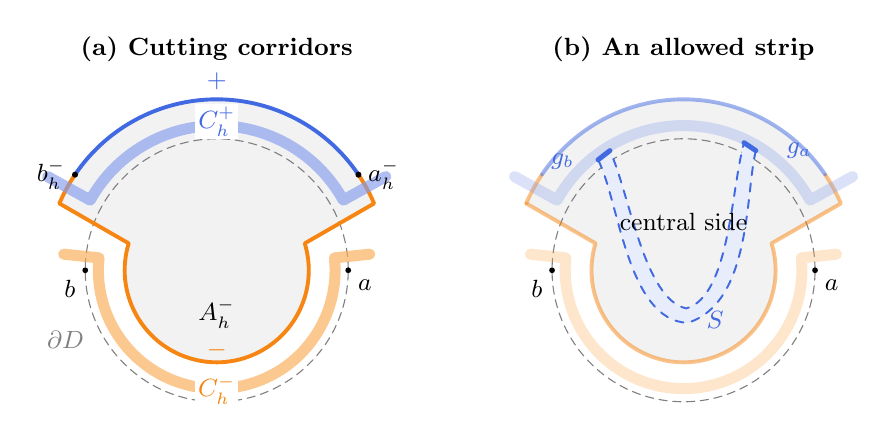
\begin{tikzpicture}[scale=1.67,line cap=round,line join=round,
  every node/.style={font=\small},
  plus/.style={draw=RoyalBlue,line width=1.4pt},
  minus/.style={draw=BurntOrange,line width=1.4pt},
  cutplus/.style={draw=RoyalBlue!65,line width=4pt,opacity=.65},
  cutminus/.style={draw=BurntOrange!65,line width=4pt,opacity=.65}]
\begin{scope}
  \node[font=\small\bfseries] at (0,1.68) {(a) Cutting corridors};
  \fill[gray!10] (23:1.30) arc[start angle=23,end angle=157,radius=1.30]
    -- (163:.70) arc[start angle=163,end angle=377,radius=.70] -- cycle;
  \draw[densely dashed,gray] (0,0) circle[radius=1];
  \draw[minus] (157:1.30)--(163:.70)
    arc[start angle=163,end angle=377,radius=.70]--(23:1.30)
    arc[start angle=23,end angle=34,radius=1.30];
  \draw[minus] (146:1.30) arc[start angle=146,end angle=157,radius=1.30];
  \draw[plus] (34:1.30) arc[start angle=34,end angle=146,radius=1.30];
  \draw[cutplus] (29:1.47)--(29:1.10)
    arc[start angle=29,end angle=151,radius=1.10]--(151:1.47);
  \draw[cutminus] (174:1.17)--(174:.90)
    arc[start angle=174,end angle=366,radius=.90]--(366:1.17);
  \node[RoyalBlue,fill=white,inner sep=1pt] at (0,1.13) {$C_h^+$};
  \node[BurntOrange,fill=white,inner sep=1pt] at (0,-.91) {$C_h^-$};
  \node at (0,-.33) {$A_h^-$};
  \node[gray] at (-1.15,-.53) {$\partial D$};
  \fill (1,0) circle[radius=.022] node[below right] {$a$};
  \fill (-1,0) circle[radius=.022] node[below left] {$b$};
  \fill (34:1.30) circle[radius=.023] node[right] {$a_h^-$};
  \fill (146:1.30) circle[radius=.023] node[left] {$b_h^-$};
  \node[RoyalBlue] at (0,1.44) {$+$};
  \node[BurntOrange] at (0,-.61) {$-$};
\end{scope}
\begin{scope}[xshift=3.55cm]
  \node[font=\small\bfseries] at (0,1.68) {(b) An allowed strip};
  \fill[gray!10] (23:1.30) arc[start angle=23,end angle=157,radius=1.30]
    -- (163:.70) arc[start angle=163,end angle=377,radius=.70] -- cycle;
  \draw[densely dashed,gray] (0,0) circle[radius=1];
  \draw[minus,opacity=.5] (157:1.30)--(163:.70)
    arc[start angle=163,end angle=377,radius=.70]--(23:1.30)
    arc[start angle=23,end angle=34,radius=1.30];
  \draw[minus,opacity=.5] (146:1.30) arc[start angle=146,end angle=157,radius=1.30];
  \draw[plus,opacity=.5] (34:1.30) arc[start angle=34,end angle=146,radius=1.30];
  \draw[cutplus,opacity=.3] (29:1.47)--(29:1.10)
    arc[start angle=29,end angle=151,radius=1.10]--(151:1.47);
  \draw[cutminus,opacity=.3] (174:1.17)--(174:.90)
    arc[start angle=174,end angle=366,radius=.90]--(366:1.17);
  \path[fill=RoyalBlue!12,draw=RoyalBlue,dashed,line width=.7pt]
    (.55,.91)..controls (.47,.60) and (.52,-.25)..(.03,-.40)
    ..controls (-.43,-.38) and (-.49,.53)..(-.65,.84)
    --(-.56,.91)
    ..controls (-.41,.58) and (-.30,-.22)..(.02,-.29)
    ..controls (.35,-.20) and (.36,.61)..(.46,.97)--cycle;
  \draw[plus,line width=1.8pt] (.55,.91)--(.46,.97);
  \draw[plus,line width=1.8pt] (-.65,.84)--(-.56,.91);
  \node[RoyalBlue] at (.88,.91) {$g_a$};
  \node[RoyalBlue] at (-.92,.83) {$g_b$};
  \node[RoyalBlue] at (.24,-.38) {$S$};
  \node at (0,.37) {central side};
  \fill (1,0) circle[radius=.022] node[below right] {$a$};
  \fill (-1,0) circle[radius=.022] node[below left] {$b$};
\end{scope}
\end{tikzpicture}
